\section{Models}
\label{sec:models}
Model is a term often used in both natural and social sciences. Unfortunately the term is not as well defined as it perhaps should be, and it will therefore here be specified what is meant by it. The approach here is based on Mario Bunge definition of a model \kanote{indsæt kilde}. According to his theory a model consists of two parts:

\begin{itemize}
\item A general theory
\item A special description of an object or system (model object)
\end{itemize}

This perception is a very general way of thinking of models and often works very well with natural and, to some degree, social sciences where experiments and models are based on an overall theory and consists of objects and systems. In social sciences, though, it often happens that the general theory is vaguely defined or even non-existent and the purpose of the model is only to observe interactions and behaviour of the systems and their objects.
To extend Bunge's theory models will here be defined as \enquote{a set of assumptions about some system} meaning everything we know about a system that we can observe or a theoretical system.
Generally there are two different types of models, static and dynamic models.


\subsection{Dynamic Models}
Dynamic models includes some form of evolution, meaning that the system changes due to some changing factor. This is often time, but can also be things like energy, as is often the case in chemistry, or alike, the only important thing is that the factor changes. Nearly all systems in natural and social sciences are dynamic models.


\subsection{Static Models}
A static model is a snapshot of a given system with objects with non-changing states. These systems are often not very representative for reality since nearly all systems changes but they can still be very useful to construct since it can be much easier to collect information and understanding through a static model. 


\section{Simulation}
We often need to create and analyse models. %Yes but for what benefit?
 For a portion of these models an analytical approach can be used, where the one can analyse the model via mathematical methods and calculate how static models will look and dynamic models evolve. This approach only works on a limited portion of the models where the system and behaviour of objects are well known and can be described mathematically. As the models become more stochastic, purely mathematical analysis begins to fall short and simulations are often used to be able to create the (often dynamic) models.

Formally simulations is defined as \enquote{a system designed to imitate another real system} \jenote{Find a better definition of a simulation}. This is a very broad definition, since real systems can be very different in their structure and further more the type of simulations also differs greatly. Generally one can distinguish between two different types of simulations, experimental and theoretical. An experimental simulation is where a real system is imitated by another real system, often smaller and/or simpler. For instance, when biologists simulate the creation of life on the back of crystals in their lab it is an experimental simulation. Theoretical simulations are simulations where a real system is imitated theoretically often on a computer or on paper. This project will focus on theoretical simulations. To further narrow the definition of a simulation used in this project, the focus will mainly be put on natural and social sciences where simulations are most often used. Within these sciences real systems can still vary a lot, but they nearly always share the property that they change state over, what is often but not necessarily, time. This is close to the definition of a dynamic model. In this respect simulations are close to a dynamic model. How this change is modelled can also vary and generally we often speak of two different paradigms; Discrete and continuous simulations.


\subsection{Continuous Simulations}
Continuous simulations are simulations that can be described with differential change. This means that
\kanote{skal gøres færdigt her}
% We make for ourselves internal images or symbols of the external objects, and we make them in such a way that the consequences of the images that are necessary in thought are always images of the consequences of the depicted objects that are necessary in nature ... Once we have succeeded in deriving from accumulated previous experience images with the required property, we can quickly develop from them, as if from models, the consequences that in the external world will occur only over an extended period or as a result of our own intervention.
\label{simulationchoise}
As an abstraction for the language to create simulations.


\subsection{Discrete Simulations}
Discrete simulations are often dictated by flows and states where the state of the whole system and subsystems are updated in discrete iterations. The systems and objects update their state each iteration. Observations in discrete simulations does not make sense during update but only before/after iterations. Figure \jenote{Make figure} shows an illustration of discrete simulations. Here we can see that the model updates instantaneous between iterations. This abstractions tend to be more useful when the simulations are better known and knowledge exists on how iterations are set in motion and the state is updated.


\subsection{Discretisation}\label{dis}

Discretisation concerns the process of transferring continuous models and equations into discrete counterparts. But whenever continuous data is discretised, there is always some amount of discretisation error.
\\\\ % Terndrup: der må findes en bedre måde at lave linjeskift
In the field of simulation, a discrete-event simulation (DES), models the operation of a system as a discrete sequence of events in time. Each event occurs at a particular instant in time and marks a change of state in the system.
Continuous simulations contrasts this in the simulation continuously tracks the system dynamics over time. Instead of being event-based, this is called an activity-based simulation; time is broken up into small time slices and the system state is updated according to the set of activities happening in the time slice. The time slices determines the granularity in time.
Another approach is process-based simulation. In this approach, each activity in a system corresponds to a separate process, where a process is typically simulated by a thread in the simulation program. In this case, the discrete events, which are generated by threads, would cause other threads to sleep, wake, and update the system state.

\kanote{Something about space granularity, memory and message sizes.}

\kanote{Number of variables considered in the simulations, is also a granularity.}

\subsubsection{Granularity}
Granularity is a qualitative measure of the ratio of computation to communication. The granularities should be chosen, accordingly with the consideration of this computation / communication ratio. Periods of computation are typically separated from periods of communication by synchronisation events.

One can say that \emph{Fine-grain Parallelism is:}

\begin{itemize}
\item Relatively small amounts of computational work are done between communication events
\item Low computation to communication ratio
\item Facilitates load balancing
\item Implies high communication overhead and less opportunity for performance enhancement
\item If granularity is too fine it is possible that the overhead required for communications and synchronisation between tasks takes longer than the computation.
\end{itemize}

and \emph{Coarse-grain Parallelism} is:

\begin{itemize}
\item Relatively large amounts of computational work are done between communication/synchronisation events
\item High computation to communication ratio
\item Implies more opportunity for performance increase
\item Harder to load balance efficiently
\end{itemize}

\subsubsection{Decomposition} \kanote{dette hører muligvis sammen med parallelism}
Decompositioning within computer science, is breaking a problem into discrete \enquote{chunks} of work that can be distributed to multiple tasks, for the computer to compute. In the decompositioning the problem, to multiple task, the designer of the solution can make use of two basic concepts, to partition the tasks in such a way that it can be parallelised, by domain and functional decomposition.

\emph{Domain decomposition} is distributing similar tasks of a problem among multiple different processors. \cref{dom} illustrates multiple similar tasks that can be parallelised, each working the on their own domain of the problem set.

\begin{figure}[htbp]\label{dom}
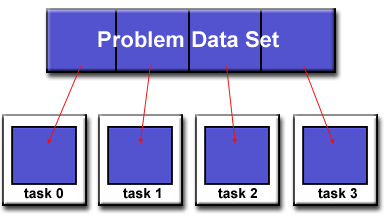
\includegraphics[width=\textwidth]{Analysis/Supercomputing/domain_decomp.png}
\caption{https://computing.llnl.gov}
\end{figure}

This is useful when working with for-loops on sets of data, if the operations of each iteration is independent of each other, the loop can easily be split up into multiple parallel tasks.

\emph{Functional decomposition} focuses on the operations performed rather than on the data manipulated by the computation. Some task differs from other in that they manipulate different data of the problem domain. This is illustrated in \cref{fun}.

\begin{figure}[htbp]\label{fun}
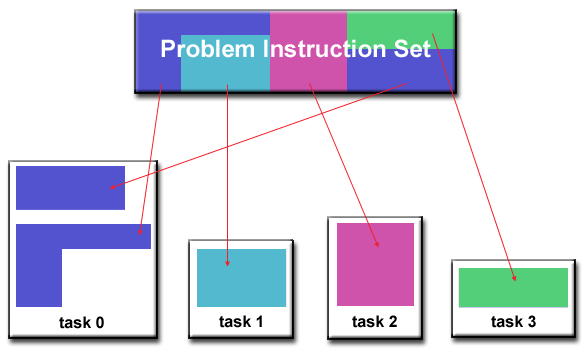
\includegraphics[width=\textwidth]{Analysis/Supercomputing/functional_decomp.png}
\caption{https://computing.llnl.gov}
\end{figure}
